\section{設計} \label{sec:design}


\sysname は,上記の設計上の課題に対するソフトウェアレベルの解決策を提供する.
コンポーネント単位で効率的に Unikernel を若返らせるために,
\sysname は各コンポーネントごとの専用のスレッドを用意し,
コンポーネントの若返りが
他のコンポーネントの実行に影響を与えるのを防ぐ.

関係のあるコンポーネントの動作状態に影響を与えるのを防ぐため,
\sysname は,ログの再生時に,再起動したコンポーネントをカプセル化する.
また,\sysname は,コンポーネント初期化後に取得したコンポーネントのメモリスナップショットを使用し,
選択的に対象のコンポーネントの状態を変化させる関数のみを実行します.


\subsection{マルチスレッド Unikernel コンポーネント}

Unikernel をコンポーネント単位で若返えらせるために,
Unikernel コンポーネントの実行について考慮する必要がある.
Unikernel は,ライブラリのように動作するため,
各コンポーネントはその機能を呼び出すスレッドコンテキストによって実行される.
Unikernel にリンクされたアプリケーションのスレッドがファイルを開くことを要求すると,
そのコンテキストは,ファイルシステム関連のコンポーネントを実行する.
本来のアプローチでは,スレッドコンテキストが対象のコンポーネントに到達したときに
そのコンポーネントを若返らせる.
この方法は,その実行に直接影響を与えるため,現在のコンテキストに関係ないコンポーネントを若返らせることができなくなる,
例えば,Unikernel にリンクされたアプリケーションがファイル関連の処理を実行している間は,
ネットワークコンポーネントを若返らせることができない.

この問題を解決するために,
\sysname はすべてのコンポーネントに専用のスレッドを割り当てて,
メッセージパッシング方式で相互に交流する.
この方式は,アプリケーションのコンテキストに対して, \sysname のコンポーネントの透過的な若返りを可能にする.
例えば,\sysname は,アプリケーションスレッドが使用していないコンポーネントを若返らせることができ,
若返りがアプリケーションの行動に影響を与えるのを防ぐ.
そして,再起動されたコンポーネントの動作状態を復元することで,
\sysname にリンクされたアプリケーションが再起動に渡って動作を継続し続けることができる.

\sysname のコンポーネントは,
それぞれ自身のデータ領域とヒープ領域を保持し,
自身に実装されている関数は,
呼び出し元コンポーネントのスレッドではなく,
自身に割り当てられている専用のスレッドによって実行される.
各スレッドは,
他のコンポーネントの関数の引数を呼び出し先のコンポーネントに渡すことにより,
その関数を呼び出し,関数の実行には,コンポーネントごとのデータ領域とヒープ領域が使われる.
通常の Unikernel では,アプリケーションがファイルを開くために,VFS (仮想ファイルシステム)のコンポーネントが公開する \textbf{open()} を呼び出す際には,
アプリケーションのスレッドコンテキストが VFS コンポーネントの \textbf{open()} へとジャンプする.
一方で, VampOS にリンクされたアプリケーションがファイルを開くには,
アプリケーションのスレッドが \textbf{open()} の引数を VFS コンポーネントに渡し,
VFS コンポーネントのスレッドが \textbf{open()} を実行する.
\sysname が引数を取り出するために,コンポーネントによって公開されたインタフェースをフックし,
呼び出し先のコンポーネントのメモリにその引数をコピーする.
関数の実行中に参照される引数は,
呼び出し元のコンポーネントのメモリにあるものではなく,
自身のメモリ上の複製されたものである.


\subsection{コンポーネントの若返り}

Unikernel のコンポーネント単位の若返りにおいて,
対象のコンポーネントの動作状態に注意を払う.
ファイルシステムやネットワークのような多くの OS サブシステムが状態を持ち,
それらの状態持つ Unikernel コンポーネントの再起動が
アプリケーションと他のコンポーネントが継続して動作させることができない.
例えば,ファイルオフセットを保持する VFS コンポーネントを若返りさせると,
ファイルオフセットが 0 に初期化されるため,
若返り後のアプリケーションのファイル操作を正しく行えなくなる.
ソフトウェア若化の観点から,
対象のコンポーネントのメモリスナップショットを再起動の直前に取得し,
動作状態を復元するのは意味がない.
なぜなら,
メモリリークやディスクリプタリーク,メモリフラグメンテーションを含む
古くなったメモリイメージが再作成されるからである.

\begin{figure}[t]
    \centering
    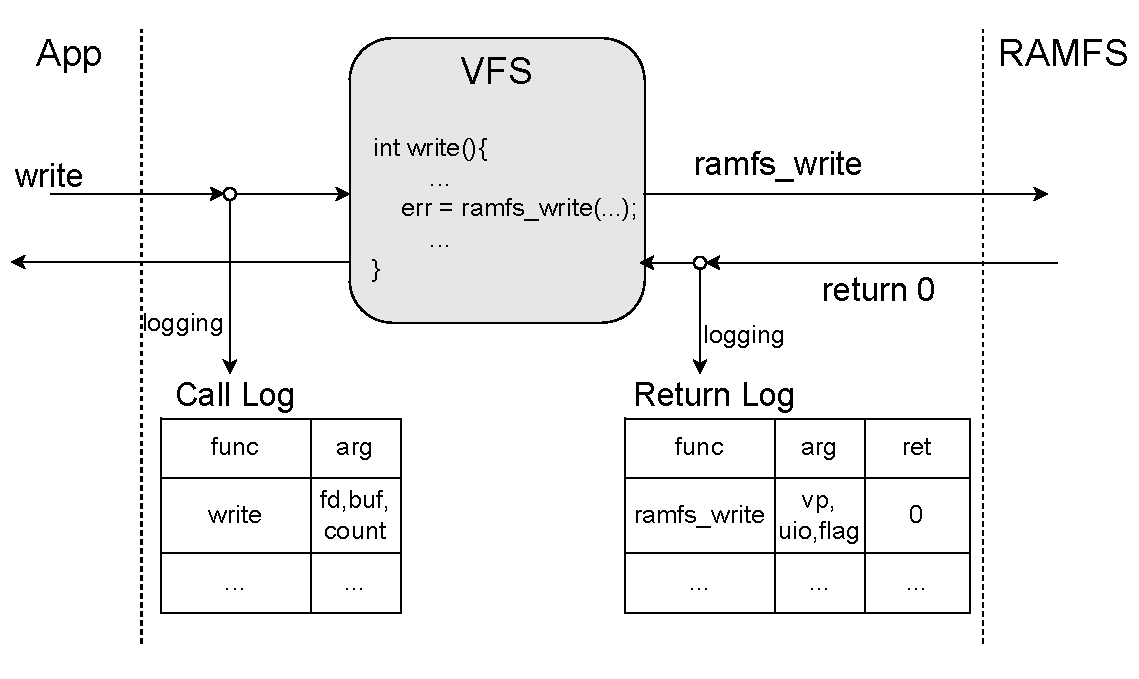
\includegraphics[width=\linewidth]{img/logging.pdf}
    \vspace{-5mm}
    \caption{コンポーネント間のインタラクションのロギング}
    \label{fig:logging}
\end{figure}

\begin{figure}[t]
    \centering
    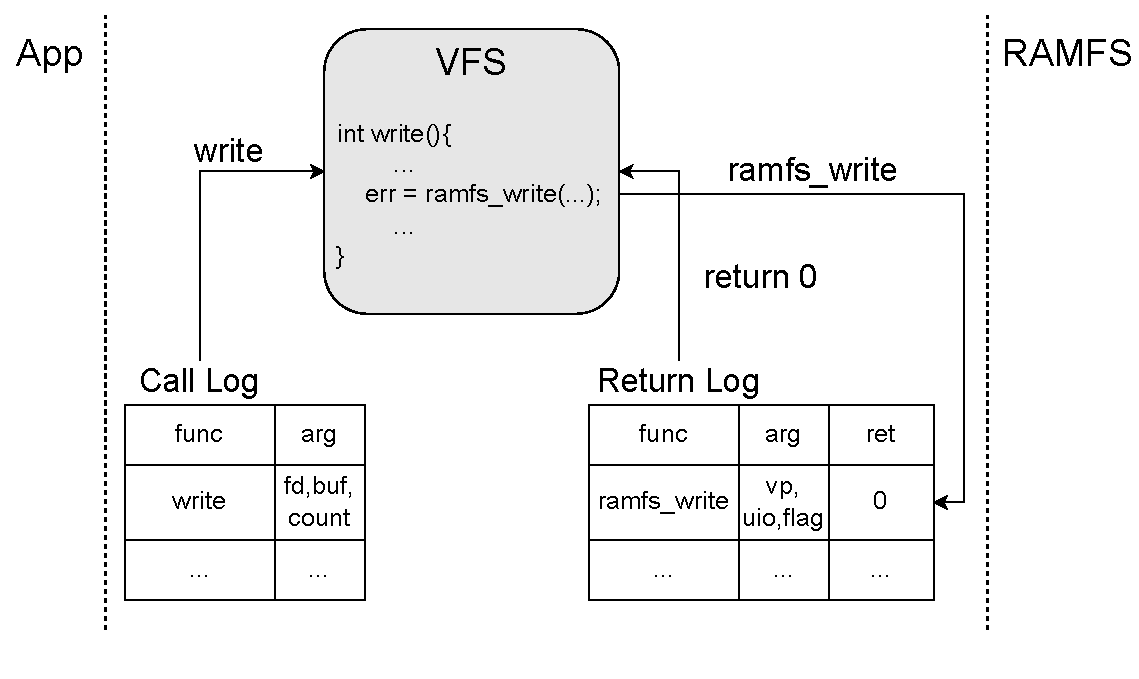
\includegraphics[width=\linewidth]{img/playlog.pdf}
    \caption{コンポーネントの復元のためのログの再生}
    \label{fig:restoration}
\end{figure}

\rr を実現するために,\sysname のコンポーネントの若返りは,
ソフトウェア若化~\cite{HuangEtAl-rejuvenation,CotroneoEtAl-rejuvenation-survey,CotroneoEtAl-Surv14}のほかに,
クラッシュやハングアップからのリカバリにも使われる.
定期的にコンポーネントの若返りを行うことで,
コンポーネントの経年劣化による不具合を未然に防ぐことで,
Unikernel の動作を安定させる.
たとえ,クラッシュやハングアップが生じたとしても,
リアクティブにコンポーネントを若返らせることで,
Unikernel が動作を継続することができる,
クラッシュは CPU トラップ時のエラーコードによって検出でき,
ハングアップは関数実行に対してタイムアウトを設けることで検出する.


状態を持つコンポーネントの若返りによって生じる不整合を防ぐため,
再起動の後に状態を持つコンポーネントの動作状態を復元する.
復元のために,\sysname は,他のコンポーネントからの対象の関数に対する関数呼び出しを記録し,
若返りの後にコンポーネントのログを再生する.
図\ref{fig:logging}は,\sysname のコンポーネント間のインタラクションのロギングを表している.
他のコンポーネントに対して透過的に若返りしたコンポーネントの動作状態を復元するために,
{\sysname} はコンポーネントが公開するインタフェースをフックし,関数呼び出しを記録した後,値を返す.
若返り前に実行されたすべての関数を再実行するのではなく,
復元の時間の短縮およびメモリリークやメモリフラグメンテーションのような老化関連のバグによるエラー状態の再現を防ぐため,
\sysname は選択的に関数を呼び出す.
\sysname は,若返りの直前の状態を復元するのに必要な関数のみを呼び出す.
具体的には,ファイル状態の読み出し(\textbf{fstat()} 関連の関数)のようなコンポーネントの状態を変更しない関数は,
呼び出されない.
また,\sysname はすでに閉じられたファイルへの操作といった
コンポーネントの現在の状態を生成しない関数は再実行しない.

さらに,\sysname では,他のコンポーネントの関数を呼び出した際の戻り値のロギングも行う.
記録した関数の戻り値は,対象のコンポーネントの状態のみを復元するのに使われる.
ログの再生による関数の実行のための単純なアプローチは,
記録されている引数で,ただ,関数を実行することである.
しかし,このアプローチでは,
若返りしたコンポーネントの動作状態を復元している間に,
他のコンポーネントの関数を呼び出すことで,
そのコンポーネントの状態を変えてしまう.
これらの状態の変化は,通常の操作ではなく,復元の操作によって引き起こされるため,
動作中のアプリケーションと対応するコンポーネントとの不整合が生じる.
復元中に若返りしたコンポーネントから他のコンポーネントに状態を変化させる関数の呼び出しを防ぐために,
他のコンポーネントの関数を呼び出すのではなく,ログに記録された値を関数の戻り値として返す.
図\ref{fig:restoration}は,\sysname のコンポーネントの状態復元の概要である.
コンポーネントの若返りの後に,\sysname は自身の状態を復元するための関数をコンポーネントに実行させる.
その際,若返り前にログに記録した他のコンポーネントの関数呼び出しの戻り値を利用させることで,
その実行による他のコンポーネントの動作状態の変化を防ぐ.



\subsection{チェックポイントベースの若返り}

シャットダウンやブート処理を行う
通常のコンポーネントの再起動は,
コンポーネント単位の若返りには適していない.
その処理は,他のコンポーネントの関数呼び出しやハードウェアの操作を含み,
コンポーネントやハードウェアの動作状態を変化させてしまう.
例えば,RAM ファイルシステム上のメモリの読み書きを行う RAMFS コンポーネントは,
シャットダウンの段階でファイルシステム内のすべての内容を消去してしまう.

この問題を解決するために,
\sysname は,
phase-based reboot~\cite{YamakitaEtAl-PBR}のアイデアを借りて,
初期化直後のコンポーネントのメモリイメージを利用する.
この phase-based reboot では,起動段階でのシステムのメモリイメージを復元することによる
若返りの効果を獲得する.
\sysname は,コンポーネント単位のチェックポイントメカニズムを提供し,
初期化されたコンポーネントのメモリスナップショットを取得する.
前の章で述べたように,
コンポーネントの若返りにおいて,
\sysname はそのメモリスナップショットの復元とログの再生を実行する.


\subsection{Intel MPK を用いたエラー伝搬の防止}

コンポーネント間のエラー伝搬の防止には,
コンポーネントの粒度でのメモリの書き込み保護が必要である.
私たちは,コンポーネント単位での保護のために Intel の Memory Protection Keys (MPK)~\cite{Intel-MPK}
を使用する.
MPK は,CPU の命令セットアーキテクチャの拡張であり,
メモリのアクセス権限を細かい粒度で高速に制御することができる.
その有用性から,
MPK を用いたセキュリティメカニズム
がいくつか提案されている\cite{ParkEtAl-libmpk,HedayatiEtAl-Hodor,Schrammel-Donky,SartakovEtAl-ASPLOS21,LefeuvreEtAl-FlexOS}.
しかし,本研究は Unikernel の \rr をテーマとしており,
エラー伝搬防止のためだけに MPK を使用し,
Unikernel への攻撃を想定しない.


MPK では,ページ単位でメモリへの読み書きを制限できる.
各ページテーブルエントリ(PTE)には 4 ビットの保護キーが設定され,
CPU コアごとの PKRU レジスタには各保護キーの設定されたページへのアクセス権限が保存されている.
メモリアクセスの度に,
メモリ管理ユニット(MMU)が対象のページの保護キーで PKRU レジスタに保存されているアクセス権限を参照し,
権限がない場合にはページフォルトが発生する.

\sysname では,MPK の保護キーを各コンポーネントに割り当て,
コンポーネント外部からの書き込みを制限することで,
コンポーネント粒度でのメモリ保護を実現する.
コンポーネントスレッドは,自身の実行するコンポーネント以外のコンポーネントのデータへの書き込みができなくなり,
ほとんどのエラー伝搬を防ぐことができる.
このメカニズムで防ぐことができないエラー伝搬については,\ref{sec:disc}章で述べる.
あるコンポーネントスレッドが書き込み可能なコンポーネントは基本的に 1 つのみであるが,
コンポーネント間で関数引数の受け渡しを実現するために,
一時的に,別のコンポーネントの保護領域への書き込み権限が与えられることもある.

